\section{Depuradores: \texttt{gdb} y \texttt{ddd}}
\label{gdb}

\definicion{Depurador}{Herramienta que permite al programador seguir la
ejecuci�n de su programa paso a paso, as� como ver el contenido de variables.}

\subsection{Depurando con \texttt{gdb}}

Para poder ejecutar un depurador sobre nuestros programas en C,
debemos especificar a gcc que incluya informaci�n de depuraci�n en los
binarios que genere. Como se vio en \ref{opciones_gcc}, en el caso de utilizar
gcc compilamos el programa 
con el modificador \texttt{-g}. 

\subsection{Depurador gr�fico: \texttt{ddd}}

DDD es un interfaz gr�fico para el depurador gdb. La principal ventaja
de ddd es la facilidad para mostrar los contenidos de las posiciones
de memoria durante la ejecuci�n de nuestro programa, como puede verse
en la siguiente captura:

\begin{figure}[H]
\begin{centering}
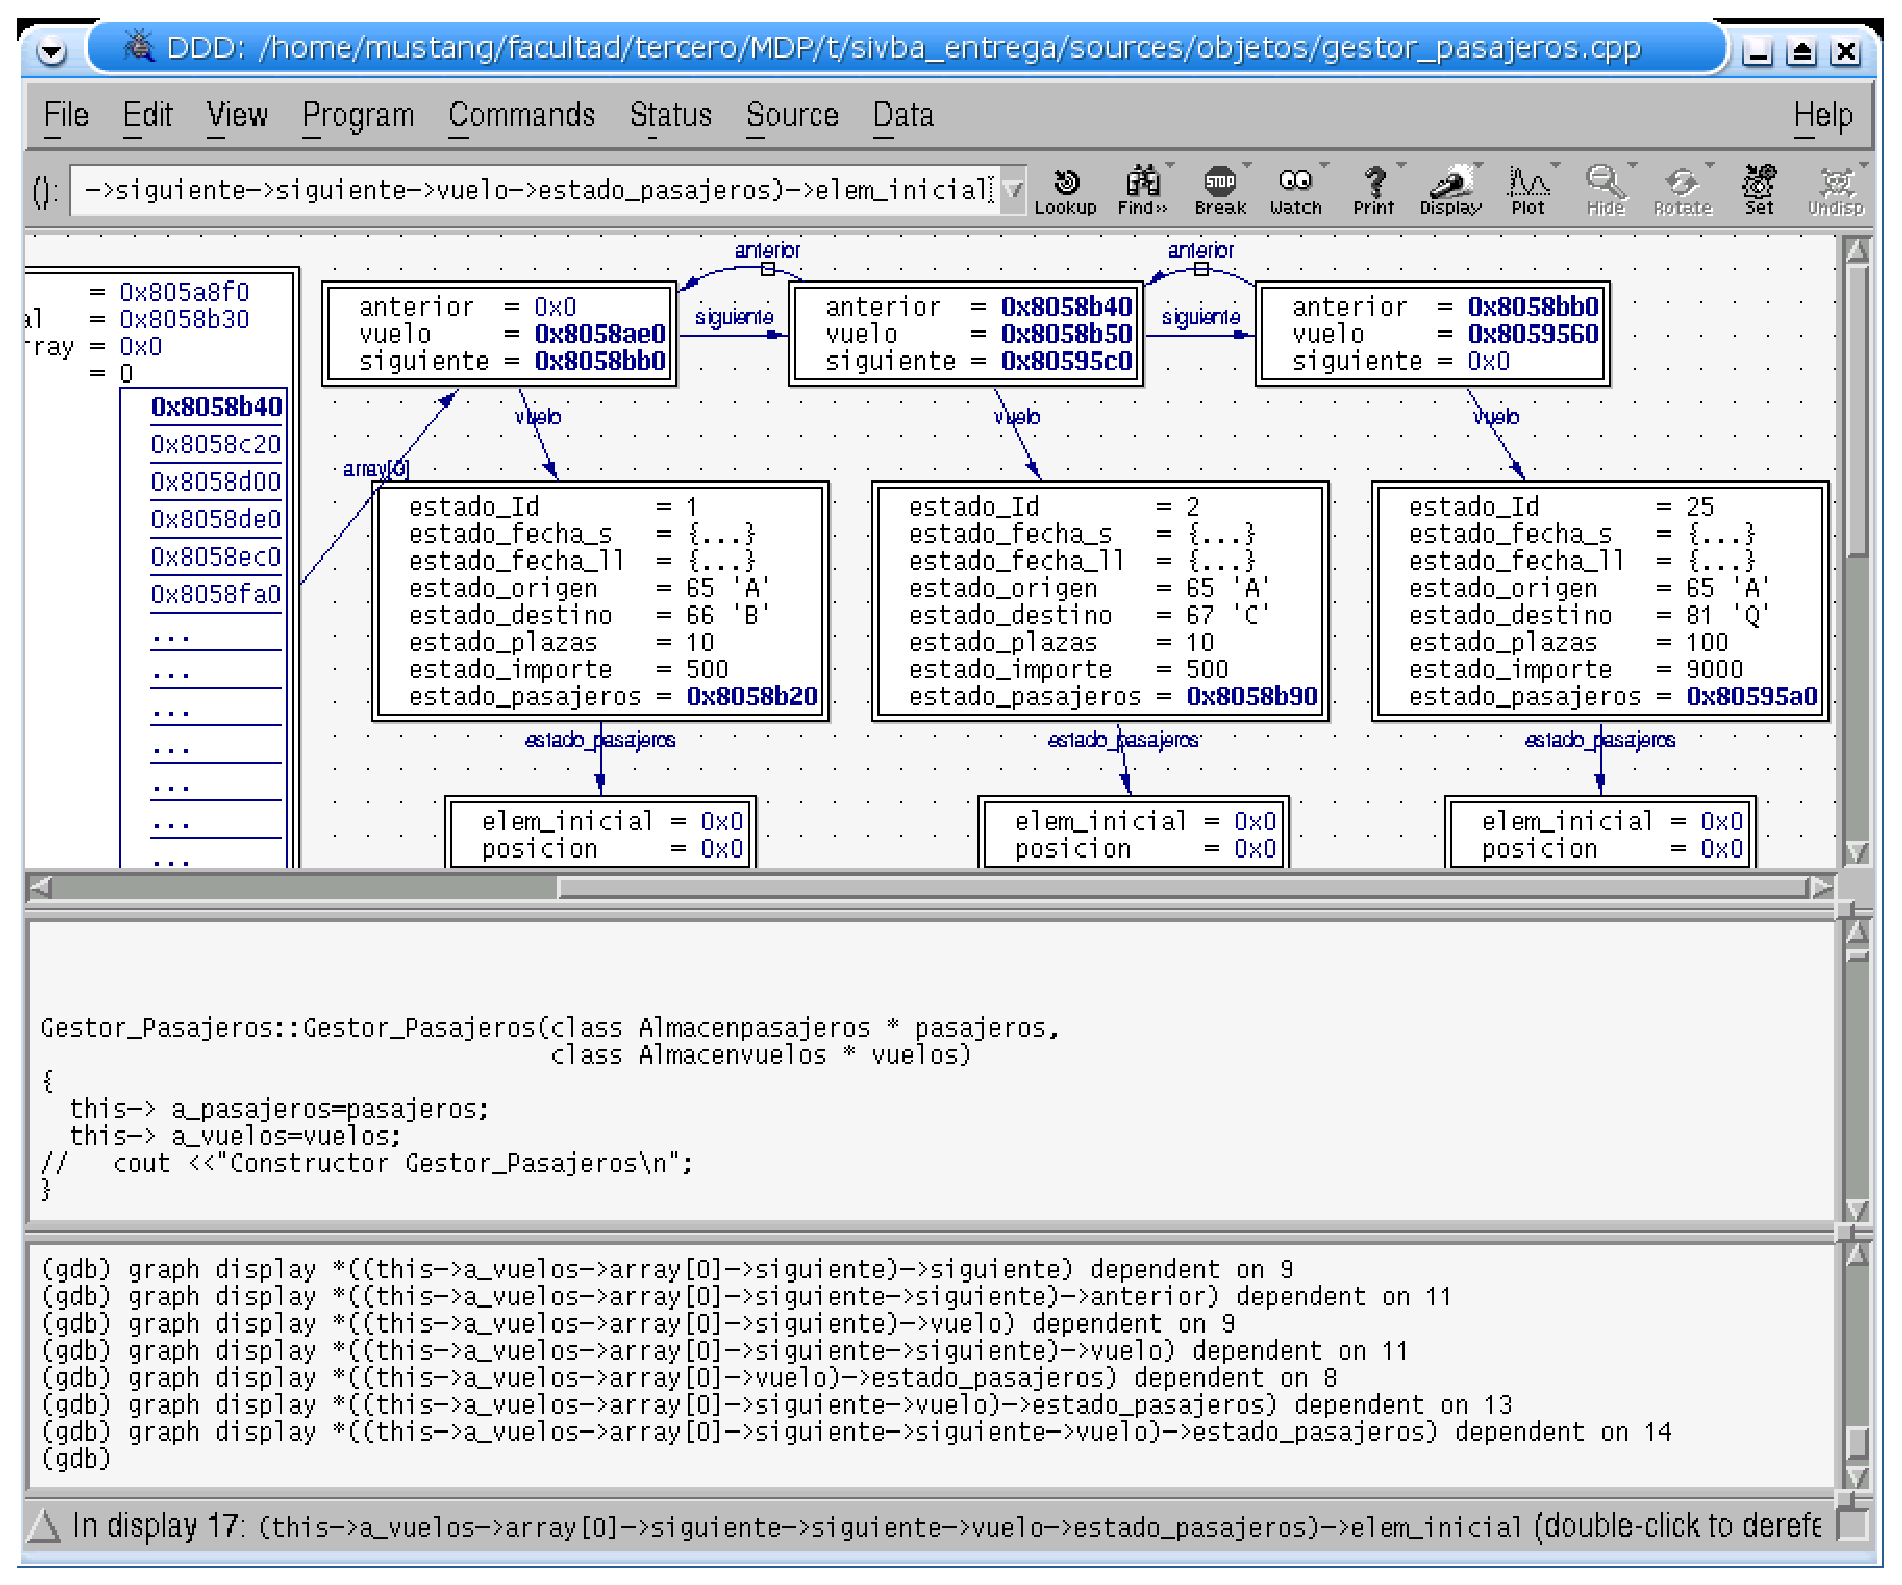
\includegraphics[width=18cm]{herramientas/ddd.eps}
\caption{DDD en accion, cadenas enlazadas}
\end{centering}
\end{figure}

\subsection{Manejo}

Para obtener una descripci�n del manejo de gdb y ddd, os remitimos a
la documentaci�n de un seminario previo de ACM: \cite{Adan}.
